%! Author = Vojta
%! Date = 21.1.2024

\chapter{Analýza}

\section{Úvod}
V této kapitole bude provedena důkladná analýza současných řešení a technologií používaných pro vývoj UI knihoven/kolekcí. Hlavním cílem analýzy je posoudit, které přístupy a technologie nejlépe vyhovují potřebám vývoje kolekce komponent určených pro \emph{framework} Nuxt, usnadňujících proces kopírování a implementace kódových úseků do cílových aplikací.

První část analýzy bude zaměřena na přehled a hodnocení stávajících řešení, která mohou sloužit jako inspirace pro kolekci. Zahrnuty budou knihovny vytvořené pro různé \emph{frameworky}, jako jsou React a Vue. Prozkoumány budou jejich vlastnosti, možnosti integrace a údržby.

Dále budou porovnány dva hlavní přístupy k integraci komponent do koncových projektů: distribuce jako samostatné balíčky (závislosti) a přímé vložení kódu do projektů. Srovnání umožní lepší pochopení dopadů každého přístupu na udržovatelnost, aktualizace a bezpečnost projektu.

Rovněž bude rozhodnuto, zda bude pro vývoj komponent preferován jazyk JavaScript nebo TypeScript, a zhodnoceno, jak volba jazyka ovlivňuje vývojový proces a integraci komponent.

Analýza závislostí jednotlivých komponent na externích knihovnách je dalším bodem, který bude zvážen, aby bylo možné maximalizovat jejich využití a minimalizovat potenciální problémy v budoucích implementacích.

Závěrem kapitoly bude definován dopad zjištěných informací na design a strukturu kolekce komponent, čímž bude kapitola připravena pro hlubší prozkoumání a evaluaci technologií a metod, které budou základem pro další vývoj.

\section{Existující řešení}

Tato část se zaměřuje na analýzu a srovnání existujících řešení ve světě UI knihoven. Tato řešení můžeme kategorizovat do dvou hlavních skupin, které se liší způsobem integrace a možnostmi úprav, což má zásadní dopad na flexibilitu a udržovatelnost výsledných aplikací.

První skupina zahrnuje knihovny poskytující sadu komponent, které jsou distribuovány jako balíčky. Tyto komponenty se do projektů přidávají jako závislosti, čímž se usnadňuje jejich správa a aktualizace. Uživatelé tyto komponenty importují do svých projektů a používají v kódu podle potřeby. Stylování těchto komponent je často omezeno na předpřipravené proměnné nebo API, které nabízí jen omezené možnosti úprav. Pokud je potřeba provést zásadnější změny v chování nebo vzhledu, může to vést k \uv{ohybání} kódu, což někdy vyústí v těžko udržovatelné řešení.

Druhá skupina se skládá z knihoven, které nejsou primárně určeny k distribuci jako balíček. Místo toho je jejich kód navržen tak, aby byl přímo zkopírován do cílového projektu, nebo jsou k dispozici prostřednictvím CLI nástrojů, které usnadňují přidání komponent jednoduchými příkazy. Tento přístup je zaměřen na maximální znovupoužitelnost a rozšiřitelnost kódu, což umožňuje uživatelům lépe přizpůsobit komponenty svým specifickým potřebám.

V následujících podsekcích bude prozkoumáno, jak tyto dva přístupy ovlivňují vývojový proces, a budou identifikovány klíčové výhody a výzvy spojené s každou skupinou. Tato analýza poskytne důležité informace pro navrhování vlastní kolekce komponent, která by měla kombinovat to nejlepší z obou světů a zároveň adresovat specifické požadavky a omezení spojená s \emph{frameworkem} Nuxt.

\subsection{Knihovny s principem balíčkování}
Knihovny s principem balíčkování představují jeden z nejběžnějších způsobů, jakým vývojáři spravují a integrují komponenty do svých webových aplikací. Tento přístup nabízí několik výhod, které ho činí atraktivním pro mnoho projektů, zejména pro ty, které vyžadují rychlý vývoj a udržování konzistence napříč velkými týmy.

Komponenty distribuované jako balíčky jsou obvykle spravovány prostřednictvím správců balíčků jako npm, yarn nebo pnpm pro JavaScriptové projekty. Tyto nástroje zjednodušují proces instalace, aktualizace a správy závislostí. Když je vydána nová verze komponenty, může být snadno aktualizována ve všech projektech, které ji využívají, což zajišťuje, že všechny aplikace mohou rychle získat přístup k novým funkcím a opravám chyb.

Použití komponent jako závislostí také podporuje konzistenci v designu a funkcionalitě. Knihovny jako Nuxt UI nebo Radix UI nabízí sadu dobře navržených komponent, které dodržují konzistentní designové prvky. To je zvláště užitečné pro týmy, které pracují na rozsáhlých projektech, protože zaručuje, že všechny komponenty v aplikaci budou vizuálně a funkčně sladěné.

Díky používání balíčkových knihoven mohou týmy výrazně snížit množství duplicitního kódu v projektu. Vývojáři nemusí vytvářet základní komponenty od nuly, ale mohou využít již existující a otestované komponenty, což šetří čas a zdroje. Tato efektivita umožňuje týmům zaměřit se na specifické aspekty svých projektů místo na znovuvynalézání běžných řešení.

Ačkoli přístup balíčkování nabízí mnoho výhod, přináší i některá omezení. Úpravy stylů a funkcionality jsou často omezeny na to, co knihovna explicitně povoluje prostřednictvím API nebo konfiguračních možností. Pokud projekt vyžaduje výrazné úpravy komponent, může být nutné \uv{ohýbat} kód, což může vést k neudržitelným a obtížně spravovatelným řešením. Tento problém je obzvláště výrazný v projektech, které vyžadují odklon od předpřipravených stylů nebo specifické funkcionality, které standardní komponenty nenabízí.

\subsubsection{Nuxt UI}
Jeden ze zástupců knihoven s principem balíčkování je Nuxt UI. Nuxt UI je relativně nová knihovna komponent, specificky navržená pro rychlou a pohodlnou tvorbu aplikací. Původně vznikla jako interní knihovna pro NuxtLabs \cite{NuxtLabs}, kteří s její pomocí vytvořili např. aplikaci Volta na pomoc vývojářům efektivně spravovat GitHub repozitáře. \cite{Volta}

Nuxt UI nabízí bohatou sadu komponent, které jsou optimalizovány pro snadné použití s \emph{frameworkem} Nuxt. Tyto komponenty jsou navrženy tak, aby poskytovaly jednotný vzhled a zároveň umožňovaly jistou míru přizpůsobení. Knihovna je postavena na principu \uv{plug and play}, což znamená, že komponenty lze snadno začlenit do projektů bez nutnosti rozsáhlé konfigurace. To umožňuje vývojářům rychle prototypovat a iterovat designy, aniž by museli obětovat kontrolu nad finálním produktem.

\begin{figure}[H]
    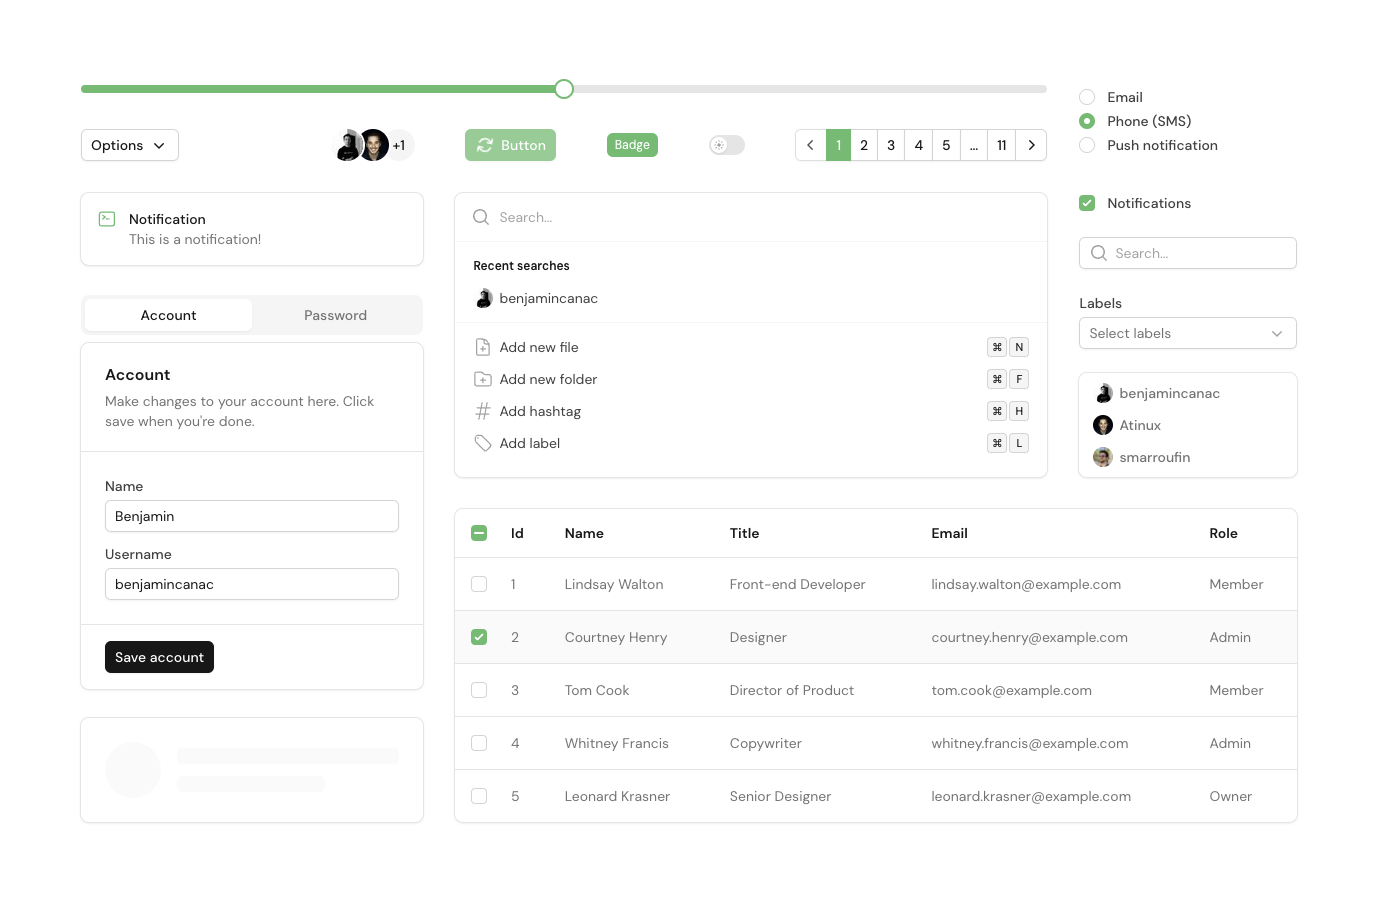
\includegraphics[width=\textwidth]{images/nuxt-ui}
    \caption{Komponenty Nuxt UI} \label{picture:nuxt-ui}
\end{figure}

\paragraph{Využití v projektech}
Nuxt UI je ideální knihovnou pro projekty, kde je primární důraz kladen na funkčnost a efektivitu vývoje, a kde výrazný individuální branding není prioritou. Tato knihovna nabízí řadu dobře promyšlených komponent, které jsou ihned připraveny k použití a pokrývají široké spektrum běžných potřeb webových aplikací.

\paragraph{Typy aplikací}
Knihovna je obzvláště vhodná pro vývoj aplikací jako jsou \emph{dashboardy}, administrační panely nebo interní nástroje, kde je důraz kladen spíše na funkčnost než na unikátní design. V těchto aplikacích je často potřeba rychle zobrazit velké množství dat přehledně a efektivně a přednastavené komponenty, jako tabulky, grafy a formuláře, které Nuxt UI nabízí, mohou výrazně urychlit vývoj a zjednodušit údržbu.

\paragraph{Robustní základ}
Pro projekty, které nevyžadují specifický vizuál, poskytuje Nuxt UI robustní základ, který minimalizuje potřebu vlastních úprav. Tím se snižují náklady na vývoj a zvyšuje se konzistence uživatelského rozhraní napříč aplikací. Uživatelé, kteří očekávají konzistentní a funkčně bohaté rozhraní, ocení, že aplikace \uv{funguje jak má} bez zbytečných komplikací nebo zpoždění způsobených potřebou výrazně přizpůsobovat základní prvky.

\paragraph{Předpřipravené šablony}
Nuxt UI nabízí řadu předpřipravených šablon, které jsou k dispozici prostřednictvím jejich \uv{Pro} plánu. Tyto šablony jsou navrženy tak, aby poskytovaly vývojářům rychlý start a efektivní nástroje pro běžné aplikace a scénáře použití. S šablonami, jako jsou administrační panely, dokumentace nebo \emph{landing page} umožňuje Nuxt UI vývojářům výrazně urychlit vývoj tím, že eliminují potřebu vytvářet často používané stránky od nuly. Každá šablona je plně responzivní, optimalizovaná pro různé typy zařízení a připravená k okamžitému nasazení. Tímto způsobem šablony nabízí nejen zrychlení vývoje, ale i zajištění vysoké úrovně kvality a uživatelské zkušenosti, které jsou důležité pro úspěšnou implementaci moderních webových aplikací. \cite{NuxtUITemplates}

\paragraph{Omezené úpravy}
Přestože knihovna Nuxt UI nabízí široké možnosti pro konfiguraci stylů svých komponent, v praxi se může ukázat, že některé typy úprav nejsou přímočaré a vyžadují větší úsilí, než bylo očekáváno. Tento problém může být zvláště patrný, když vývojáři chtějí provést specifické změny, které nejsou přímo podporovány základním API knihovny. V důsledku toho mohou být nuceni používat obcházení standardních metod, což může vést k méně udržitelnému kódu a potenciálně k narušení konzistence a funkčnosti aplikace.

Jedním z příkladů, kde mohou vývojáři narazit na obtíže, je pokus o radikální změnu vzhledu komponent, které Nuxt UI poskytuje jako standardní. Ačkoliv knihovna umožňuje základní úpravy jako změny barev, fontů a odsazení prostřednictvím předdefinovaných proměnných, hlubší zásahy do \emph{layoutu} nebo chování komponent mohou vyžadovat přímé zásahy do CSS nebo struktury komponent. To může být časově náročné a komplikované, zejména pokud se tyto změny snaží zachovat responzivitu a přístupnost komponent.

\paragraph{Figma Kit}

Knihovna nabízí také Figma Kit, který umožní designérům snadno vytvářet prototypy a designové systémy s komponentami Nuxt UI. Tím se zajišťuje, že design a implementace jsou vzájemně sladěny a že výsledná aplikace bude vizuálně konzistentní a uživatelsky přívětivá. \cite{NuxtUIFigma}

\paragraph{Hodnocení}

\begin{itemize}
    \item \textbf{Výhody}
    \begin{itemize}
        \item Velké množství komponent
        \item Propracované styly
        \item Připravené pro použití
    \end{itemize}
    \item \textbf{Nevýhody}
    \begin{itemize}
        \item Omezené možnosti rozšíření
        \item Složitější úpravy stylů
        \item Složité úpravy funkcionality
    \end{itemize}
\end{itemize}

\clearpage

% https://www.radix-ui.com/primitives/docs/overview/introduction
\subsubsection{Radix UI}
Radix UI představuje \emph{open source} knihovnu UI komponent, která je zaměřena na tvorbu kvalitních a přístupných designových systémů a webových aplikací.
Jde především o Radix Primitives, což jsou nízkoúrovňové UI komponenty s důrazem na přístupnost a možnost úprav vývojářů s cílem vytvoření vlastní knihovny.
Tyto komponenty lze využívat buď jako základní vrstvu designového systému nebo je postupně implementovat do stávajících projektů. \cite{RadixUIPrimitives}

\begin{figure}[H]
    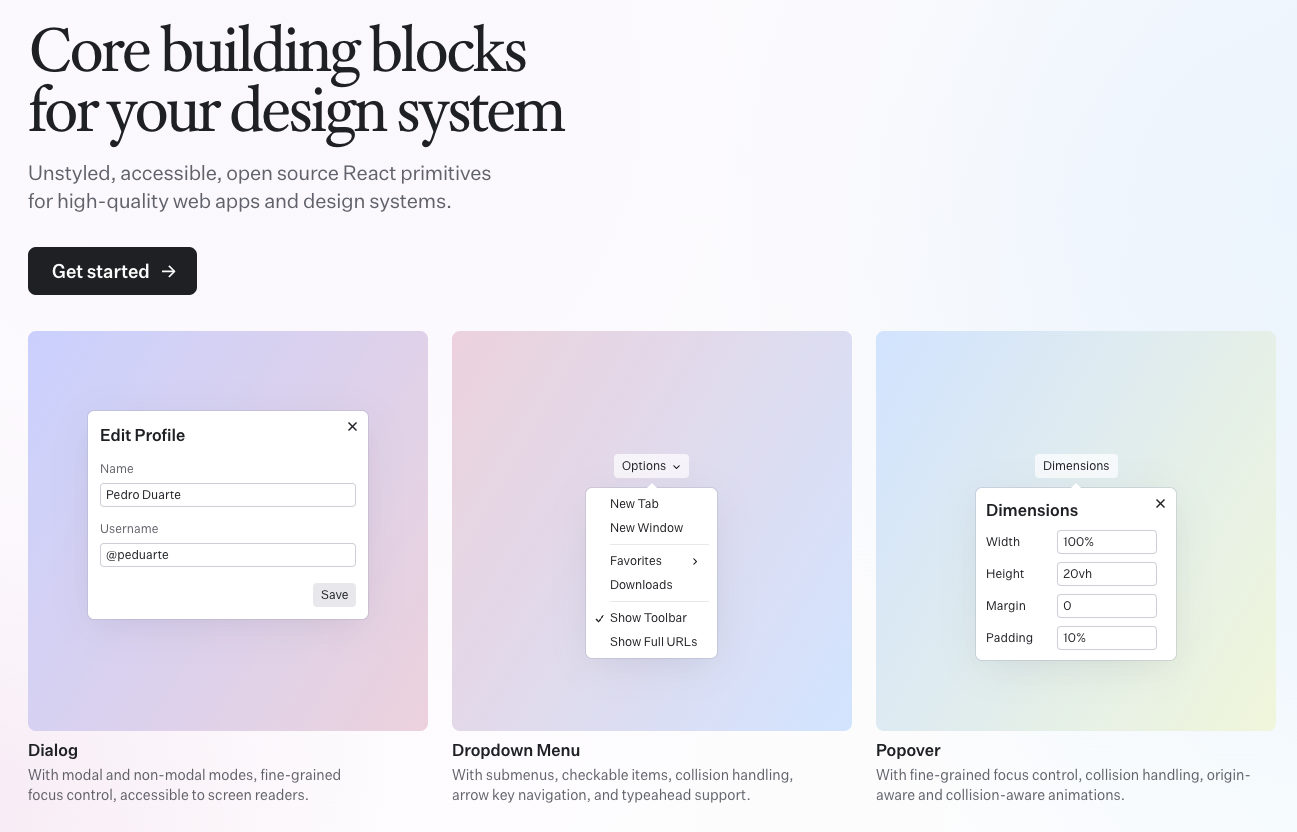
\includegraphics[width=\textwidth]{images/radix-ui}
    \caption{Primitivní komponenty Radix UI} \label{picture:radix-ui}
\end{figure}

Jedním z hlavních rysů Radix UI je jeho důraz na přístupnost. Všechny komponenty jsou navrženy tak, aby splňovaly standardy WAI-ARIA a poskytovaly bezproblémovou podporu pro pohyb pomocí klávesnice a asistenční technologie. Tento přístup zajišťuje, že aplikace vyvinuté s Radix UI budou přístupné širšímu spektru uživatelů, což je důležité pro vytváření inkluzivních digitálních produktů.

Radix UI se odlišuje od mnoha jiných UI knihoven tím, že neobsahuje žádné předdefinované styly. Místo toho poskytuje primitivní komponenty, které lze použít jako základní stavební bloky pro vlastní komponenty. Tyto primitivní komponenty jsou navrženy tak, aby byly co nejvíce konfigurovatelné, což umožňuje vývojářům vytvářet unikátní uživatelská rozhraní bez omezení specifickými designovými rozhodnutími.

Radix UI nabízí širokou nabídku komponent, které pokrývají vše od základních prvků, jako jsou tlačítka a přepínače, až po složitější kontrolní prvky, jako jsou dialogová okna a \emph{dropdown} menu. Každá komponenta je navržena tak, aby poskytovala optimální uživatelskou zkušenost a byla snadno integrovatelná do různých projektů. To vývojářům umožňuje rychle sestavit funkcionalitu, kterou potřebují, zatímco si udržují úplnou kontrolu nad chováním a vzhledem aplikace.

Na druhou stranu jedna z hlavních nevýhod Radix UI spočívá v tom, že vývojáři musí vynaložit značné úsilí při vytváření konkrétních komponent, protože Radix UI poskytuje pouze primitivní komponenty, které slouží jako základní stavební bloky. Komponenty neobsahují žádné předdefinované styly ani komplexní funkcionality, což znamená, že na vývojářích leží úkol implementovat vizuální design, interakce a další specifické aspekty, které jsou potřebné pro jejich projekt. Tento přístup vyžaduje pokročilé znalosti v CSS a správné porozumění nejlepším praktikám přístupnosti a interaktivity, aby bylo možné plně využít potenciál primitivních komponent. Ačkoliv tento model poskytuje maximální flexibilitu, může být také časově náročný a může zpomalit vývoj, zejména ve fázích, kdy je potřeba rychle prototypovat, nebo když tým nemá dostatek zdrojů na detailní vývoj každé komponenty od základů.

\paragraph{Hodnocení}

\begin{itemize}
    \item \textbf{Výhody}
    \begin{itemize}
        \item Velké množství primitivních komponent
        \item Promyšlený koncept
    \end{itemize}
    \item \textbf{Nevýhody}
    \begin{itemize}
        \item Velká část implementace spadá na vývojáře
    \end{itemize}
\end{itemize}

\subsection{Knihovny s principem vlastnění kódu}
Knihovny s principem vlastnění kódu poskytují vývojářům jedinečný přístup k použití a úpravě komponent ve svých projektech. Tento model se liší od běžnějších knihoven tím, že vývojáři mají možnost přímo manipulovat s kódem komponent, což jim umožňuje provádět hluboké a specifické změny, které by jinak byly obtížné nebo nemožné.

Hlavní výhodou tohoto přístupu je extrémní flexibilita. Vývojáři nejsou omezeni předdefinovaným API nebo funkčností komponenty. Místo toho mohou přímo upravit zdrojový kód komponenty, aby lépe vyhovoval specifickým potřebám jejich aplikace. Tato schopnost je obzvláště cenná v projektech, kde je potřeba pečlivě laděná funkcionalita, nebo když standardní komponenty jednoduše neodpovídají požadovaným designovým nebo technickým specifikacím.

Projekty vyžadující vysokou míru přizpůsobení mohou zvláště těžit z modelu vlastnění kódu. Tento přístup je také vhodný pro vývojové týmy, které mají silné znalosti a zkušenosti s daným programovacím jazykem a \emph{frameworkem}, neboť jim umožňuje plně využít své dovednosti bez omezení.

Přestože poskytuje vysokou míru kontroly, vlastnění kódu také přináší určité výzvy. Správa vlastního kódu může být časově náročnější, protože tým musí zajišťovat údržbu a aktualizace komponent, což by jinak mohlo být delegováno na externí knihovny. Tento model také může vést k větší fragmentaci kódu, pokud každý projekt vyžaduje unikátní úpravy, což komplikuje možnost sdílení kódu mezi projekty nebo při práci ve velkých týmech. Tento problém se dá v rámci \emph{frameworku} Nuxt řešit pomocí vlastních modulů, které umožňují sdílení kódu mezi projekty - např. v rámci monorepozitáře.

\subsubsection{shadcn/ui}
Shadcn/ui je inovativní \emph{open source} knihovna UI komponent, která je navržena tak, aby vylepšila webový vývoj, zejména pro projekty využívající React.
Hlavní předností této knihovny je její lehkost, díky čemuž se snadno integruje do projektů bez nutnosti zatěžujících závislostí. Knihovna staví
zejména na komponentách Radix UI, které kladou důrat na přístupnost, což zajišťuje, že komponenty jsou inkluzivní a použitelné pro všechny uživatele. \cite{ShadcnUI}

\begin{figure}[H]
    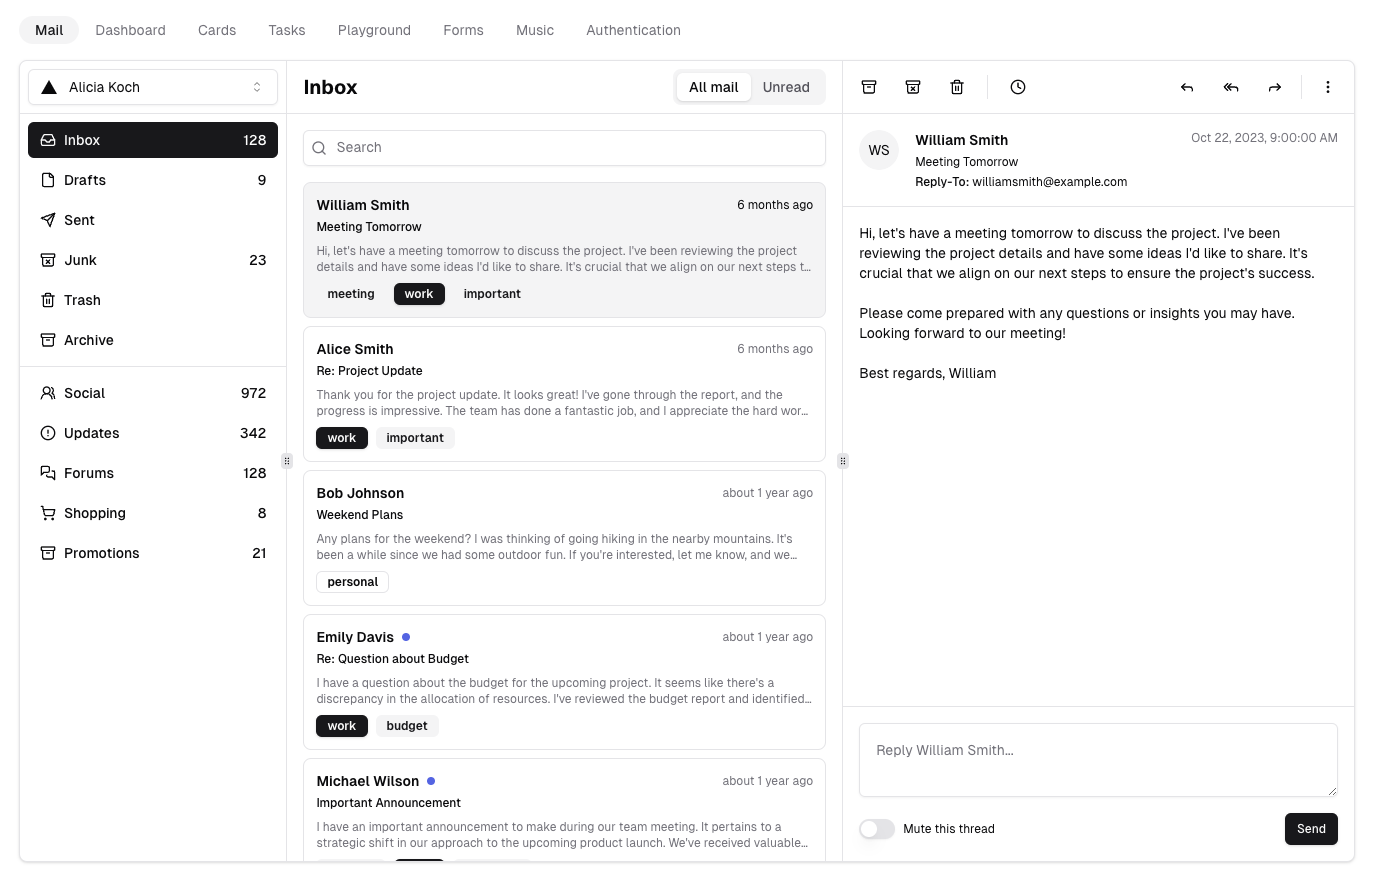
\includegraphics[width=\textwidth]{images/shadcn}
    \caption{Emailový klient vytvořený pomocí shadcn/ui} \label{picture:shadcn}
\end{figure}

Několik hlavních myšlenek autora knihovny shadcn/ui, proč je lepší kód vlastnit (kopírovat), než používat balíčky \cite{ShadcnUI}:

\begin{itemize}
    \item Smyslem je poskytnout vlastnictví, kontrolu nad kódem a možnost rozhodovat o tom, jak budou komponenty použity a stylizovány.
    \item Začít s nějakými rozumnými výchozími nastaveními, a poté přizpůsobit součásti potřebám projektu.
    \item Jednou z nevýhod balíčkování komponent do npm balíčku je, že styl je spojen s implementací. Styl komponent by měl být oddělen od jejich implementace.
\end{itemize}

Na rozdíl od Radix UI nemusí vývojáři věnovat tolik času vývoji komponent, protože jsou již předpřipravené (složené z primitivních komponent Radix UI). Také mají možnost upravit kód komponent, což jim umožňuje přizpůsobit je specifickým potřebám jejich projektu. Tento přístup kombinuje výhody distribuovaných knihoven s flexibilitou vlastního kódu, což umožňuje vývojářům rychle upravovat komponenty podle potřeby.

Další významnou součástí knihovny shadcn/ui je integrace s \emph{frameworkem} Tailwind CSS, který poskytuje efektivní a přívětivé prostředí pro vývojáře preferující tento CSS \emph{framework} orientovaný na utilitu. Výhody Tailwind CSS jsou popsány v kapitole věnované technologiím. Tato integrace umožňuje snadnou úpravu a rozšíření stylů. Shadcn/ui vyniká svou snadnou použitelností a detailní kontrolou nad komponentami. Vývojáři mohou přímo přistupovat ke zdrojovému kódu jednotlivých komponent, což umožňuje jejich efektivní úpravy pro specifické případy užití a požadavky aplikace.

Shadcn/ui také nabízí CLI, který usnadňuje práci s knihovnou komponent. Umožňuje vývojářům inicializovat projekt nebo rychle přidávat komponenty přímo z příkazové řádky. Vývojáři mají také možnost porovnat změny mezi jejich kódem a kódem knihovny, což usnadňuje sledování a správu změn v kódu.

Podobně jako Nuxt UI, také shadcn/ui nabízí knihovnu komponent ve Figmě. Na rozdíl od Nuxt UI nebyla vytvořena autory, ale členem open-source komunity. \cite{ShadcnUIFigma}

\paragraph{Hodnocení}

\begin{itemize}
    \item \textbf{Výhody}
    \begin{itemize}
        \item Jednoduché úpravy
        \item Kód vlastní uživatel
    \end{itemize}
    \item \textbf{Nevýhody}
    \begin{itemize}
        \item Omezená funkcionalita
        \item Větší objem spravovaného kódu
    \end{itemize}
\end{itemize}

\section{Proces aktualizace}
Proces aktualizace komponent se výrazně liší mezi knihovnami s principem balíčkování a knihovnami s principem vlastnění kódu. U knihoven s principem balíčkování je proces aktualizace relativně jednoduchý a efektivní. Vývojáři mohou snadno aktualizovat komponenty na nejnovější verzi pomocí správce balíčků, což zajišťuje, že všechny závislosti jsou správně spravovány a kompatibilní. Tento přístup minimalizuje riziko konfliktů v kódu a umožňuje týmům rychle reagovat na opravy chyb nebo získat nové funkce bez nutnosti zásadně přepisovat existující kód (za předpokladu zachování rozhraní komponent).

Na druhé straně, u knihoven s principem vlastnění kódu, kde vývojáři přebírají základní komponenty a adaptují je podle svých potřeb, není aktualizace tak přímá. Protože tyto komponenty jsou často značně upraveny a integrovány přímo do kódu aplikace, neexistuje jednoduchý mechanismus pro jejich aktualizaci prostřednictvím správce balíčků. Místo toho mohou projekty vyžadovat vlastní řešení, jako je vývoj vlastního CLI nástroje, který by pomáhal spravovat a aktualizovat tyto upravené komponenty. Alternativní možností je, že aktualizace se jednoduše nebudou implementovat, protože jejich komponenty jsou specificky navrženy pro konkrétní použití a nevyžadují pravidelné aktualizace, jaké jsou běžné u standardních knihoven komponent.

\section{TypeScript vs JavaScript}

V současné době, kdy technologie neustále pokračují ve svém vývoji, je volba vhodného programovacího jazyka velmi důležitá. Mezi nejpopulárnější a široce používané programovací jazyky v oblasti webu patří JavaScript a jeho nadstavba TypeScript. Každý z nich přináší specifické výhody i potenciální komplikace. Tato sekce se zaměří na porovnání těchto dvou technologií, aby bylo možné učinit informované rozhodnutí o tom, který jazyk je pro náš projekt nejvhodnější.

\subsection{JavaScript}
JavaScript je dynamický skriptovací jazyk, který byl původně navržen pro manipulaci s webovými stránkami, ale postupem času se jeho využití rozšířilo i do mnoha dalších oblastí včetně serverových aplikací, desktopových aplikací, a dokonce i programování hardwaru. Jako jazyk běžící přímo v prohlížeči má JavaScript nezastupitelnou roli ve vývoji front-endu. \cite{JavaScript}

\subsubsection{Výhody}

\begin{description}
    \item[Univerzálnost a dostupnost] JavaScript je podporován všemi hlavními prohlížeči bez potřeby jakéhokoliv doplňku.
    \item[Velká komunita a ekosystém] Existuje obrovské množství knihoven, \emph{frameworků} a nástrojů, které usnadňují vývoj v JavaScriptu.
    \item[Flexibilita] JavaScript umožňuje různé styly programování (procedurální, objektově orientované, funkcionální), což dává vývojářům svobodu ve výběru přístupu k řešení problémů.
\end{description}

\subsubsection{Nevýhody}

\begin{description}
    \item[Bez typové bezpečnosti] Jazyk je dynamicky typovaný, což může vést k chybám za běhu, které jsou obtížně odhalitelné během vývoje.
\end{description}

\subsection{TypeScript}
TypeScript je nadstavba JavaScriptu vyvinutá společností Microsoft, která přidává statickou typovou kontrolu a další funkce zaměřené na zlepšení organizace kódu a jeho udržitelnosti. TypeScript je plně kompatibilní s JavaScriptem, což znamená, že jakýkoli platný JavaScriptový kód je také platným TypeScriptovým kódem. \cite{TypeScript}

\subsubsection{Výhody}

\begin{description}
    \item[Statická typová kontrola] Přidává bezpečnost typů na úrovni kompilace, což pomáhá odhalit chyby dříve, usnadňuje \emph{refactoring} a zvyšuje čitelnost kódu.
    \item[Podpora pro velké projekty] S funkcemi jako jsou rozhraní a generika, TypeScript lépe podporuje vývoj větších a technicky složitějších aplikací.
    \item[Vylepšená nástrojová podpora] Integrace s vývojovými prostředími (IDE) poskytuje lepší nástroje pro automatické dokončování kódu a navigaci.
\end{description}

\subsubsection{Nevýhody}

\begin{description}
    \item[Náročnější na naučení] Přechod a následné používání TypeScriptu může vyžadovat dodatečnou práci v podobě přidání typových anotací a konfigurace. Také může být pro nové uživatele náročnější se naučit nové koncepty a syntaxi.
\end{description}

\subsection{Porovnání}
V nedávné minulosti se některé velké \emph{open source} projekty, jako je například Svelte nebo Drizzle, rozhodly přejít z TypeScriptu zpět na JavaScript. Tento trend vyvolal diskuzi o tom, který jazyk je pro vývoj knihoven lepší. Je několik klíčových faktorů, které je třeba zvážit při rozhodování mezi JavaScriptem a TypeScriptem.

Projekty, které přešly z TypeScriptu na JavaScript, stále používají JSDoc definice pro generování typů. Všechny tyto projekty byly velké, složité, a potřebovaly vyřešit problémy s definicí typů, které v rámci takto velkých projektů mohou vyžadovat velké množství práce. \cite{DitchingTypescript}

\subsubsection{Výhody přechodu na JSDoc}

\begin{itemize}
    \item Bez TypeScriptu se zmenší velikost balíčků.
    \item Možnost přejít na zdrojový kód kliknutím na import funkce usnadňuje úpravy a ladění \emph{frameworku}.
    \item Pro zobrazení změn není potřeba propojovat repozitář, kompilovat v režimu sledování nebo rozumět mapování mezi zdrojovým a distribučním kódem.
\end{itemize}

\subsubsection{Nevýhody přechodu na JSDoc}

\begin{itemize}
    \item Nutnost používat JSDoc pro psaní typů, což není tak příjemné jako psaní v TypeScriptu.
\end{itemize}

\begin{listing}[H]
    \caption{JSDoc komentáře \cite{JSDocExample}}
    \label{lst:jsdoc-example}
    \begin{code}[js]
/**
* Returns the sum of a and b
* @param {number} a
* @param {number} b
* @param {boolean} retArr If set to true, the function will return an array
* @returns {(number|Array)} Sum of a and b or an array that contains a, b and the sum of a and b.
*/
function sum(a, b, retArr) {
    if (retArr) {
        return [a, b, a + b];
    }
    return a + b;
}
    \end{code}
\end{listing}

Na druhou stranu pro koncové aplikace je TypeScript stále lepší volbou, protože poskytuje výhody statické typové kontroly, které mohou výrazně snížit počet chyb a zvýšit kvalitu kódu. \cite{FireshipTypescript}

Vzhledem k tomu, že většina kódu se dostane přímo do rukou vývojářů, bude lepší použít TypeScript, se kterým se lépe pracuje v koncových aplikacích. Pro knihovny, které jsou určeny k širokému použití jako balíčky, může být lepší použití JavaScriptu, protože to zjednoduší vývoj knihovny z hlediska typování atd., a zmenší velikost balíčků. Pro použití kolekce tedy bude povinná závislost na TypeScriptu.

Může se zdát, že jako ideální možnost se nabízí použití JavaScriptu v kombinaci s JSDoc a vygenerováním typů do balíčku (např. \emph{@types/v-moravec-ui}). Bohužel toto řešení není možné bez nutnosti udržovat dvojnásobek zdrojového kódu, protože integrace do koncových aplikací musí být v TypeScriptu. Kód s JSDoc komentáři by byl nedostatečný pro využití všech výhod TypeScriptu.

\section{Závislosti na knihovnách třetích stran}
Využití závislostí třetích stran v procesu vývoje komponent může přinést řadu výhod, zvláště když je důraz kladen na efektivitu a dostupnost. Knihovny poskytující přístupné UI prvky jsou zajímavou možností, která umožňuje urychlit proces implementace bez ztráty kontroly nad funkcionalitou a stylováním. Pro React je zajímavá knihovna Radix UI, avšak její Vue verze je spravována komunitou a nedosahuje takové kvality, jako ta původní. Knihovna, která je dostupná pro oba \emph{frameworky}, se jmenuje Headless UI.

Přestože knihovny třetích stran mohou nabídnout robustní a funkční komponenty, je důležité, aby vývojáři udrželi plnou kontrolu nad funkcemi a stylováním svých aplikací. To znamená, že i když jsou základní komponenty převzaty, měli by být schopni je dále upravovat a přizpůsobovat tak, aby odpovídaly specifickým požadavkům a estetickým preferencím projektu. Tyto požadavky Headless UI splňuje a dává tedy smysl jej využít. Tím odpadá potřeba implementovat nízkoúrovňové rozhraní, ale vývojáři budou stále mít vysokou kontrolu nad funkcionalitou a vizuálem díky přímému přístupu k zdrojovému kódu.

Aktualizace využitých knihoven mají pak vývojáři na starosti sami. Na jednu stranu to znamená, že jim přibude určitá zodpovědnost při aktualizaci, na druhou stranu mohou využít nové funkce a opravy chyb bez nutnosti čekat na oficiální aktualizaci knihovny (oproti knihovnám s principem balíčkování, kde by bylo potřeba vytvářet vlastní \emph{patch} nebo \emph{fork}).

\section{Závěr}
Tato kapitola poskytla komplexní přehled stávajících UI knihoven a technologií, které ovlivňují vývoj a implementaci komponent. Důkladné srovnání přístupů založených na balíčkování a vlastnictví kódu odhalilo výhody a nevýhody každého z nich. Zvážení aspektů jako udržovatelnost, aktualizace a flexibilita vedlo k rozhodnutí o preferenci přístupu s vlastnictvím kódu pro maximální přizpůsobení a kontrolu.

Dále bylo provedeno porovnání programovacích jazyků TypeScript a JavaScript, přičemž byl zdůrazněn přínos statické typové kontroly TypeScriptu pro větší projekty a jeho dopad na kvalitu kódu. Nakonec, analýza závislostí na knihovnách třetích stran, jako je Headless UI, poukázala na potenciál pro urychlení vývoje, a zároveň zdůraznila nutnost zachování kontroly nad funkcemi a stylováním.

Získané poznatky z analýzy poskytují pevný základ pro návrh a implementaci sbírky znovupoužitelných UI komponent, která bude efektivní, flexibilní a přizpůsobitelná specifickým potřebám vývojářů.

